\section{Обзор существующих решений}
Существуют различные способы задания шаблонов для форматирования. Далее рассматриваются некоторые из них, а так же приводится описание структуры проекта, в рамках которого будет реализовываться дополнительный функционал.

\subsection{Средства форматирования в IDE}
Интегрированные среды разработки предоставляют средства для форматирования программного кода. Рассмотрим их на примере IDE IntelliJ IDEA\footnote{\texttt{http://jetbrains.com/idea}}. Необходимый стиль кодирования (СК) задается с помощью различных настроек форматтера. Среди них:
\begin{itemize}
  \item настройка размера и типа отступа (табуляция или пробелы);
  \item принудительная расстановка фигурных скобок;
  \item расположение простых блоков на одной или нескольких строках.
\end{itemize}

На рис.~\ref{fig:intellijSettings} приведен диалог задания параметров форматирования в IntelliJ IDEA.

\begin{figure}[h!]
	\centering
	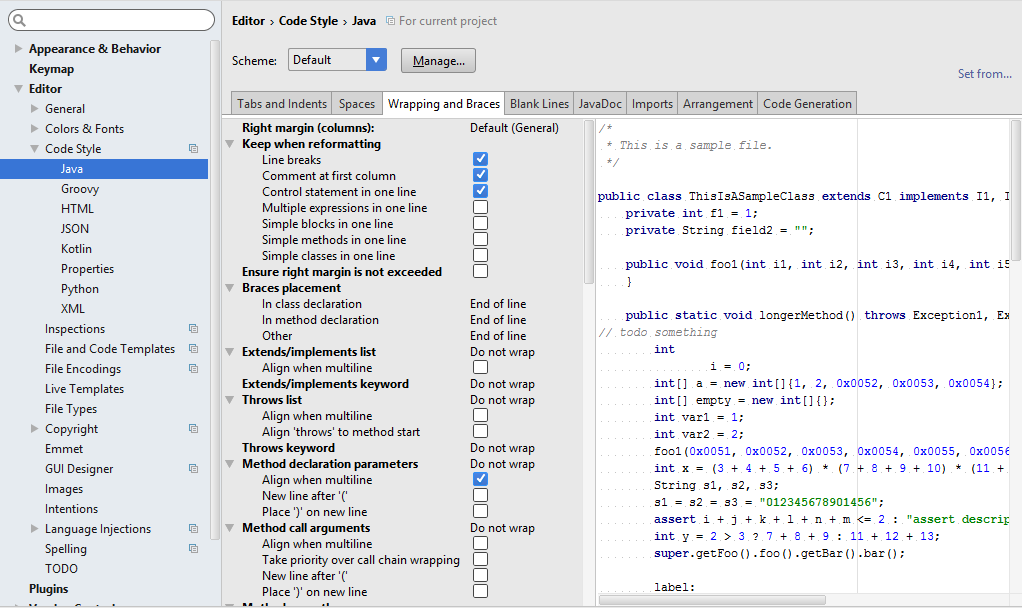
\includegraphics[width=\textwidth]{Ozernykh/images/intellijSettings}
	\caption{Окно настройки форматтера IntelliJ IDEA}
	\label{fig:intellijSettings}
\end{figure}

Однако у встроенных форматтеров есть недостатки. Во-первых, с помощью упомянутых настроек нельзя выразить нестандартный СК (см. рис.~\ref{fig:unusualCC}). 
Во-вторых, стиль кодирования, указанный в настройках, будет применен ко всем блокам некоторого типа, независимо от их форматирования. 
Иногда имеет смысл поддерживать различные варианты форматирования для блоков одного типа в рамках проекта. %есть дальше пример. Сослаться?

\begin{figure}[h]
	\centering
	\lstinputlisting[language=Java]{Ozernykh/codes/unusualCC.txt}
	\caption{Нестандартный СК для языка С}
	\label{fig:unusualCC}
\end{figure}

\subsection{Stratego/XT}
Stratego/XT\footnote{\texttt{http://strategoxt.org}}~--- язык и набор инструментов для преобразования программ. Язык предоставляет правила переписывания, описывающие базовые шаги преобразования программы~\cite{stratego:xt}.
Одно из этих правил изображено на рис.~\ref{fig:rewriting}.

\begin{figure}[h]
	\lstinputlisting[language=Haskell]{Ozernykh/codes/desugar.txt}
	\caption{Правило для развертки блока While}
	\label{fig:rewriting}
\end{figure}

Преобразование программы производится путем одного или нескольких применений этих правил к абстрактному синтаксическому дереву (АСТ) (рис.~\ref{fig:stratego}), а затем "красивой" печати этого дерева согласно некоторым правилам форматирования. Одно из правил преобразования АСТ в текст изображено на рис.~\ref{fig:strategopp}.

\begin{figure}[h]
	\centering
	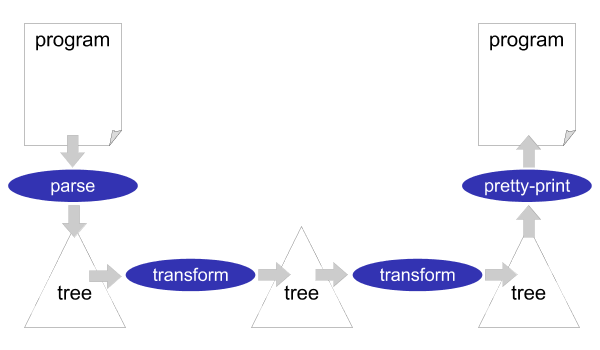
\includegraphics[width=0.7\textwidth]{Ozernykh/images/pipe.jpg}
	\caption[Преобразование программ в Stratego/XT]{Преобразование программ в Stratego/XT\footnotemark}
	\label{fig:stratego}
\end{figure}

\footnotetext{\texttt{http://releases.strategoxt.org/}}


\begin{figure}[h]
	\centering
	\lstinputlisting[language=Haskell]{Ozernykh/codes/strategopp.txt}
	\caption{Правило для преобразование АСТ в текст в Stratego/XT}
	\label{fig:strategopp}
\end{figure}


Недостатками этого подхода являются, во-первых, необходимость владения синтаксисом языка Stratego, во-вторых, нужна отдельная среда разработки (к примеру, IntelliJ IDEA и Visual Studio не имеют плагина, позволяющий работать со Stratego/XT), в-третьих, данный подход имеет единые правила форматирования структур одного типа, а значит, не может поддерживать различные стили форматирования для них.

\subsection{Принтер-плагин для IntelliJ IDEA}
Другой метод задания шаблонов представляет собой принтер-плагин для IntelliJ IDEA, позволяющий форматировать исходный текст по образцу. Образцом является некоторый репозиторий, содержащий код с желаемым форматированием.
%даиграмму?
Пользователь выбирает файлы проекта-образца и целевой файл для форматирования. Каждый файл представляется в виде дерева разбора, состоящего из элементов классов типа \lstinline[language=Java]{PsiElement}~\cite{intellij:plugdev}, например, \lstinline[language=Java]{PsiIfStatement} (оператор ветвления), \lstinline[language=Java]{PsiExpressionStatement} (выражение). Из этих элементов извлекаются шаблоны 
% * <igor.ozernykh@gmail.com> 21:32:55 20 May 2015 UTC+0300:
% Смотри картинку с иерархией
форматирования с помощью метода \lstinline[language=Java]{getAndSaveTemplate()} 
класса \lstinline[language=Java]{PsiElementComponent}. Эти шаблоны будут 
использоваться принтером (\lstinline[language=Java]{Printer}) для изменения 
форматирования целевого файла.

Затем принтер получает на вход целевой файл и к каждому элементу дерева 
применяет функцию% \lstinline[language=C++]{applyTmplt()}
, которая строит 
\lstinline[language=Java]{FormatSet}, набор, состоящий из различных вариантов 
форматирования, построенных исходя из извлеченных шаблонов. Из этого набора
выбирается лишь один вариант форматирования, и происходит перепечатывание
этого элемента дерева разбора с учетом нового форматирования.
Взаимодействие классов изображено на рис.~\ref{fig:hierarchyPP}.

\begin{figure}[h!]
	\centering
	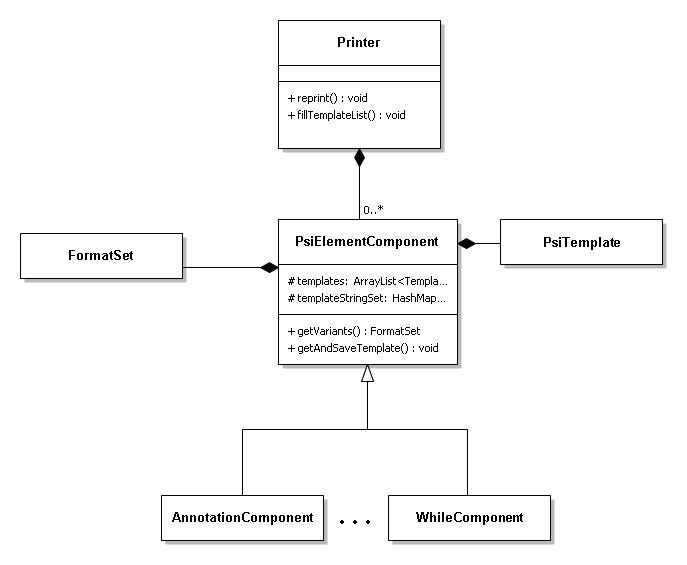
\includegraphics[width=\textwidth]{Ozernykh/images/hierarchyPP}
	\caption{Основные классы принтер-плагина}
	\label{fig:hierarchyPP}
\end{figure}

Рассмотренные способы задания шаблонов не могут поддерживать различные стили форматирования для элементов одного типа, а так же не имеют возможности задания шаблонов в интерактивном режиме. 

